\documentclass{standalone}
\usepackage{tikz}

\begin{document}

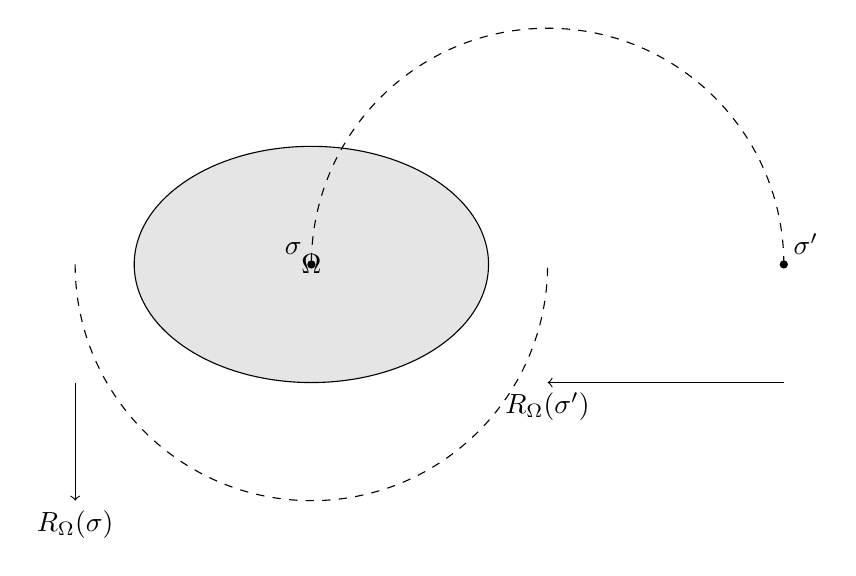
\begin{tikzpicture}[scale=1.5]
    % Define the domain Omega
    \fill[gray!20] (0,0) ellipse (1.5 and 1);
    
    % Draw the domain Omega
    \draw (0,0) ellipse (1.5 and 1);
    
    % Draw the circle R_Omega(sigma)
    \draw[dashed] (-2,0) arc (180:360:2);
    
    % Draw the circle R_Omega(sigma')
    \draw[dashed] (4,0) arc (0:180:2);
    
    % Label the domain Omega
    \node at (0,0) {$\Omega$};
    
    % Label the points sigma and sigma'
    \fill (0,0) circle (1pt) node[above left] {$\sigma$};
    \fill (4,0) circle (1pt) node[above right] {$\sigma'$};
    
    % Label the radius R_Omega(sigma)
    \draw[->] (-2,-1) -- (-2,-2) node[below] {$R_\Omega(\sigma)$};
    
    % Label the radius R_Omega(sigma')
    \draw[->] (4,-1) -- (2,-1) node[below] {$R_\Omega(\sigma')$};
\end{tikzpicture}

\end{document}